Two user interfaces were developed for the model. The first one, named \textit{TextGUI}, a pure textual output displaying all the statistical data for the simulation as well as generating text files with the sequence of coverage data during the run. This was used comprehensively to analyze and compare the performance of different algorithms. 

The second one, named \textit{MainWindow}, provided graphical representation of the balloons at each step. The design was very rudimentary and was developed purely for debugging purposes at early stages of the project. Seeing the initial movements of the heard of balloons gives a clear image of the behaviour of the model and whether it is working properly or not. The simulation window gives the user an opportunity to take a single step, or up to 200 steps at at time, using the slider object.


\begin{figure}[H]
    \centering
    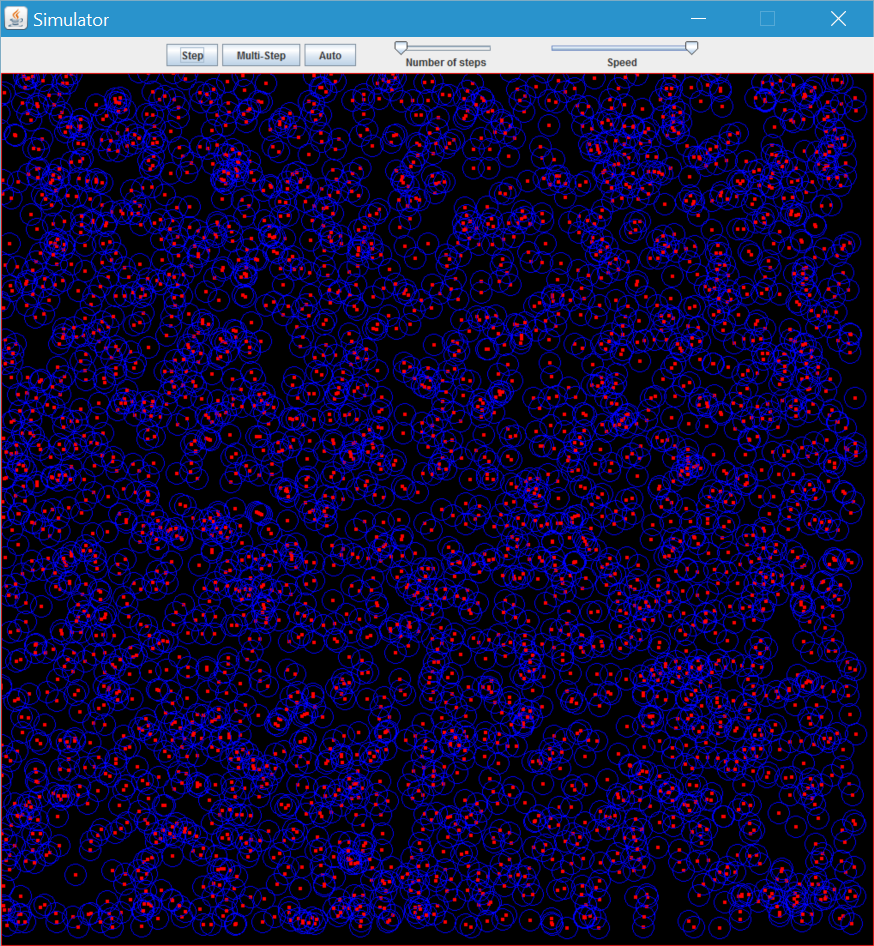
\includegraphics[width=0.7\textwidth]{graphics/MainWindow.png}
\caption{Simulator}
\label{fig:mainwindow}
\end{figure}

The speed of the simulation can be controlled with another slider object. This second interface is not bound to the model parameter NUMBER\_OF\_STEPS so it will run until stopped. This is useful to see how an algorithm works during long simulations. In this project a visual representation is often the fastest measure of quality of an algorithm. 